\subsection{Model \#2: fixed planets and primaries, varying secondaries}
\label{sec:model_2}

\begin{figure}[!tb]
    \centering
    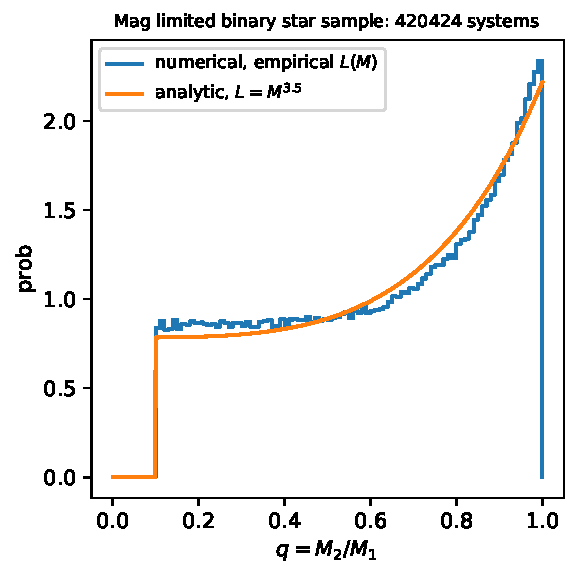
\includegraphics[width=0.6\textwidth]{figures/q_distribn_mag_limited.pdf}
    \caption{
        The distribution of the mass ratio for a magnitude limited sample of 
        binary stars. The underlying mass ratios are drawn from a uniform 
        distribution in a volume-limited sample, quite similar to that of 
        Raghavan 
        et al. (2010)'s Fig. 13.
        The entire bias can be understood analytically 
        (Eq.~\ref{eq:Malmquist_bias}).
        {\bf todo: make y axis label p(secondary with q).}
    }
    \label{fig:q_distribn_mag_limited}
\end{figure}

Our binary-twin model provides a simple estimate of binarity's systematic 
effects, but perhaps it is too simple.
We begin introducing realism by first letting the light ratio $\ell = L_2/L_1$ 
vary across the binary population.
It does so because the underlying mass ratio $q=M_2/M_1$ varies.
We keep the primary mass fixed as $M_1$, which is also the mass of all single 
stars.

We parametrize the distribution of binary mass ratios in a volume-limited 
sample as a power law: $p(q)\propto q^\beta$.
For binaries with solar-type primaries\footnote{
Duchene and Kraus (2013), fitting all the multiple systems of Raghavan et al. 
(2010)'s Fig 16, find $\beta = 0.28\pm0.05$ for $0.7<M_\star/M_\odot<1.3$.
Examining only the binary systems of Rhagavan et al 2010, Fig 16, the 
distribution seems roughly uniform, $\beta \approx 0$, except for a claimed 
excess of twin binaries with $q\approx 1$, and an obvious lack of $q<0.1$ 
stellar companions.
}, $\beta$ is probably between 0 and 0.3.
We further assume that stars are a one-parameter family, $R \propto M \propto 
L^{1/\alpha}$, so that a drawn value of $q$ determines everything about a 
secondary.

The rate density in this model, $\Gamma(r,q)$, is the sum of the rate 
densities for each system type:
\begin{equation}
\Gamma(r,q)
=
\delta(r_p) \times 
\frac{N_0 Z_0 + N_1 Z_1 + N_2 Z_2 p_2(q)}{N_{\rm tot}}
\label{eq:model2_rate_density}
\end{equation}
where $p_2(q)$ is mass-ratio dependent shape function in secondaries. A fully 
general approach would parametrize $p_2(q)$ as a power law, $p_2(q) \propto 
q^\gamma$. For simplicity we will always take $\gamma=0$, the uniform case.
%We have written $\Gamma$ in terms of the mass ratio instead of the 
%secondary star's radius for convenience ($q$ and $R_2$ are interchangeable).
The interpretation of $Z_i$ is still ``the number of planets per star of 
type $i$'', but now for secondaries this must include a marginalization 
over both the mass ratio and the planet radius.

There is also a Malmquist bias in Eq.~\ref{eq:model2_rate_density}, hidden 
away in the numbers of selected stars.
This is because the selected sample at a fixed planet radius and period is 
magnitude-limited.
Given a binary, the probability of drawing a mass ratio $q$ in a 
magnitude-limited sample scales as
\begin{equation}
p({\rm draw\ }q | {\rm system\ is\ binary}) \propto q^\beta (1+q^\alpha)^{3/2}
\label{eq:Malmquist_bias}
\end{equation}
where $q^\beta$ is the volume-limited probability of drawing a binary of mass 
ratio $q$, and the latter term is the Malmquist bias.
We show the magnitude-limited mass ratio distribution for the $\beta=0$ case 
in Fig.~\ref{fig:q_distribn_mag_limited}.
We emphasize that in Monte Carlo simulations of transit surveys, it is 
important to draw binaries from the correctly biased mass-ratio distribution 
(e.g., Bakos et al 2012, Sullivan et al 2015, Guenther et al 2017).

The occurrence rate corresponding to Eq.~\ref{eq:model2_rate_density}'s rate 
density for specific mass ratios of interest $q_{\rm min} < q < q_{\rm 
max}$ is then
\begin{equation}
\Lambda|_{r_p,q_{\rm min},q_{\rm max}} = 
\frac{N_0 Z_0 + N_1 Z_1 + N_2 Z_2 f_2}
{N_{\rm tot}},
\end{equation}
for
\begin{equation}
f_2 \equiv
\int_{q_{\rm min}}^{q_{\rm max}} p_2(q) \,{\rm d}q,
\end{equation}
where $p_2(q)\propto q^\gamma$, and must be normalized to unity.


\paragraph{What do the observers ignoring binarity infer?}
As a reminder, the binary-ignoring observers compute an apparent rate density 
by correcting the number of detections per star for the transit probability 
and the detection efficiency.
In this process, they make the following errors:
\begin{enumerate}
\item They assume that they have selected $N_0+N_1$ stars, while they have 
actually selected $N_0+N_1+N_2$.
%
\item They assume that every star within the maximum selected distance is 
searchable.
This is true for single stars.
For binaries, the actual detection efficiency is the ratio of the number of 
searchable stars to the number of selected stars.
For primaries,
\begin{equation}
p_{\rm det,1} = \left(\frac{d_{\rm det,1}}{d_{\rm sel}}\right)^3
= \mathcal{D}_1^3 = (1+q^\alpha)^{-3},
\label{eq:model_2_p_det_1}
\end{equation}
where we have assumed that all single stars and primaries have the same 
properties, and have used $\ell = q^\alpha$.
For secondaries,
\begin{equation}
p_{\rm det,2} = \left(\frac{d_{\rm det,2}}{d_{\rm sel}}\right)^3
= \mathcal{D}_2^3 \left(\frac{R_1}{R_2}\right)^6
    \left(\frac{T_{\rm dur,2}}{T_{\rm dur,1}}\right)^{3/2} 
= (1+q^{-\alpha})^{-3} q^{-5},
\label{eq:model_2_p_det_2}
\end{equation}
where subscripts `1' and `2' correspond to primaries and secondaries, and we 
used the scaling relation $T_{\rm dur}\propto \rho_\star^{-1/3} \propto 
R_\star^{2/3}$.
%
\item They assume a transit probability for all stars of $p_{\rm tra} = 
R_\star/a$. 
For planets orbiting secondaries at fixed period, the true transit probability 
is $q^{2/3} p_{\rm tra}$, since the secondaries have smaller radii and masses.
%
\item The true planetary radii $r$ are interpreted as apparent radii $r_a$.
In binaries, the apparent radii depend on whether the host is the primary or 
secondary:
    \begin{align}
    r_a
    &=
    \left.
    \begin{cases}
    r_p (1+q^\alpha)^{-1/2} & \text{for } i=1,\ {\rm primary} \\
    r_p (1+q^{-\alpha})^{-1/2} q^{-1}, & \text{for } i=2,\ {\rm secondary}.
    \end{cases}
    \right.
    \label{eq:model2_ra}
    \end{align}
    The factor of $q^{-1}$ for the secondary case accounts for the observer 
    assuming all transit signals come from stars of fixed size.
\end{enumerate}

To write the apparent rate density as a function of the apparent 
radius $r_a$, we marginalize out the planet period, semimajor axis, and 
stellar radius (or equivalently the mass ratio, for binaries):
\begin{equation}
\Gamma_a(r_a) =
\frac{N_0}{N_0+N_1} Z_0 \delta(r_p)
+
\frac{N_1}{N_0+N_1} \left( Z_1 I_1(r_a)
+
Z_2 I_2(r_a) \right).
\label{eq:model2_Gamma_a}
\end{equation}
The ratio of primaries to singles, $\mu=N_1/N_0$, is now less than 
that of Model \#1 (cf. Eq.~\ref{eq:mu_definition}). This is because a 
distribution of light 
ratios $\ell$ leads to a distribution of maximum selected distances. 
Integrating over the mass ratios from $q=0$ to $1$, one finds a
dimensionless integral
\begin{equation}
\mu \equiv \frac{N_1}{N_0} = \frac{\rm BF}{1 - {\rm BF}} \left(2^{3/2} - 
\int_{1}^{\sqrt{2}} u^2 (u^2 -1)^{1/\alpha} \,{\rm d}u\right).
\label{eq:mu_model_2}
\end{equation}

Given a binary fraction, Eq.~\ref{eq:mu_model_2} fully specifies the 
``weights'' in Eq.~\ref{eq:model2_Gamma_a}.
The $I_1(r_a)$ and $I_2(r_a)$ terms are found by marginalizing over the joint 
distribution of apparent radius and mass ratio:
\begin{align}
I_i(r_a) &= 
\int_0^1 p({\rm has\ detected\ planet}, r_a, q | {\rm star\ is\ type\ }i)
    \,{\rm d}q,
\quad
{\rm for}\ i\in\{1, 2\}, \\
&=
\int_0^1 
    p({\rm has\ detected\ planet} | r_a, q, {\rm star\ is\ type\ }i) 
    \nonumber\\
    &\quad\quad\quad\quad\times p(r_a | q, {\rm star\ is\ type\ }i)
    \,p(q | {\rm star\ is\ type\ }i)
\,{\rm d}q.
\end{align}
The first term is the detection efficiency; the second is a $\delta$-function 
of the apparent radius; the last is the mass ratio distribution given by 
Eq.~\ref{eq:Malmquist_bias}.
An analytic solution can be found for $i=1$.
For $i=2$ there is no analytic solution, because evaluating the integral 
requires imposing the constraint that $r_a  = r_p 
(1+q^{-\alpha})^{-1/2}q^{-1}$. This equation can be re-written
\begin{equation}
\left(\frac{r_p}{r_a}\right)^2 = q^2 + q^{-\alpha + 2},
\end{equation}
which has no analytic solution for $q(r_a)$ except for special values of 
$\alpha$, the mass-luminosity exponent.
For $\alpha=3.5$, our nominal case, semianalytic solutions do exist.
However, since our main interest is in understanding the qualitative behavior 
of the solutions, we derive a limiting case, and then proceed 
numerically.

\begin{comment}
The analytic solution for $i=1$ is something like
\begin{equation}
I_1(r_a) = \frac{1}{\mathcal{N}_1} \left(\frac{r_p}{r_a}\right)^{-3}
\left( \left(\frac{r_p}{r_a}\right)^2 -1  
    \right)^{\frac{\gamma+\beta}{\alpha}},
\quad {\rm for}\ r_p/\sqrt{2} < r_a < r_p,
\end{equation}
where $\mathcal{N}_1$ is the normalization term of the binary mass ratio 
distribution (Eq.~\ref{eq:model_2_p_2}): $\mathcal{N}_1 = \int_0^1 
q^{\gamma+\beta} (1+q^\alpha)^{3/2} {\rm d}q$.
\end{comment}




\paragraph{Limiting case of rate density correction}
Recall that the rate density correction factor, $X_\Gamma$, is the ratio of 
the apparent to true rate densities.
We consider a ``nominal model'' in which the stellar population is similar to 
Sun-like stars in the local neighborhood:
${\rm BF}=0.44$, $\alpha=3.5$, $\beta=0$.
Our default assumption is also that the occurrence of planets is independent 
of stellar mass ($\gamma=0$), so secondaries have the same occurrence rate as 
primaries and single stars.
Under these assumptions, the true rate density is
\begin{equation}
\Gamma(r) \approx \delta(r_p) \left( Z_0 + Z_1 + 
Z_2 \right) / 3,
\label{eq:model2_Gamma_r}
\end{equation}
where the coefficients of $1/3$ are accurate to within one percent of the true 
coefficients.
Ignoring binarity, the observer finds an apparent rate density
\begin{equation}
\Gamma_a(r) = c_0 Z_0 \delta(r_p)
             +c_1 Z_1 I_1(r_a)
             +c_2 Z_2 I_2(r_a),
\label{eq:model2_Gamma_a_r}
\end{equation}
for $c_0\approx 0.49$, and the coefficients $c_1, c_2$ unknown.
%171011_integrals.nb $c_1\approx 0.32$
We can evaluate the correction term at $r=r_p$, since $\lim_{r_a\rightarrow 
r_p} I_i(r_a)=0$ for $i\in\{1,2\}$:
\begin{equation}
X_\Gamma(r=r_p) \approx \frac{3c_0 \Lambda_0}{\Lambda_0+\Lambda_1+\Lambda_2}.
\end{equation}
If all the $Z_i$'s are equal, $X_\Gamma(r=r_p)\approx0.49$.
If there are no planets around the secondaries, $X_\Gamma(r=r_p)\approx0.74$.

\begin{figure}[!t]
    \centering
    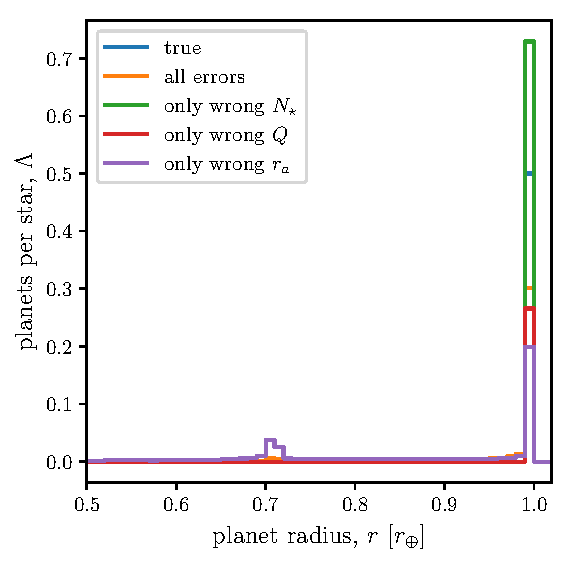
\includegraphics[width=.6\textwidth]{figures/errcases_rate_density_vs_radius_model_2.pdf}
    \caption{
        Inferred planet occurrence rates as a function of planet radius in 
        Model 
        \#2.
        This model has fixed planets and primaries, but varying secondaries.
    }
    \label{fig:errcases_model_2_linear}
\end{figure}
\begin{figure}[!h]
    \centering
    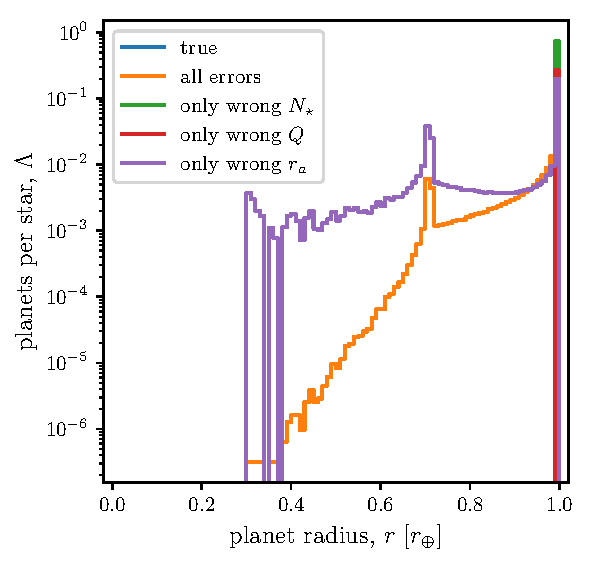
\includegraphics[width=.6\textwidth]{figures/errcases_rate_density_vs_radius_logs_model_2.pdf}
    \caption{
        Same as Fig.~\ref{fig:errcases_model_2_linear}, but with logarithmic 
        $y$-axis, and different $x$ scale.
    }
    \label{fig:errcases_model_2_log}
\end{figure}

\paragraph{Numerical approach}
To maintain simplicity, we develop a Monte Carlo program to simulate our 
toy transit surveys.
The program generates a stellar population, assigns planets to the stars, and 
then calculates which planets are detectable.
It then computes the apparent and true planet occurrence rates as a function 
of planet radius.
This is discussed in detail below, and our implementation is available 
online\footnote{\url{https://github.com/lgbouma/binary_biases}}.

First, the user must specify the free parameters that describe the 
stellar and planetary population. These values include the binary fraction, 
and the true planet occurrence rates around single stars, primaries, and 
secondaries (the $Z_i$'s; recall Eq.~\ref{eq:rate_density_shape}).
There is also an arbitrary absolute number of selected stars.

Once the user specifies the free parameters, the program constructs a 
population of selected stars.
Each selected star is assigned a type (single, primary, secondary), a 
binary mass ratio (if it is not single), and the property of whether it is 
``searchable''.
The relative number of binaries to primaries is set by 
Eq.~\ref{eq:mu_model_2}.
The mass ratios are drawn from the appropriate magnitude-limited distribution 
(Eq.~\ref{eq:Malmquist_bias}).
If it is single, a selected star is assumed to be searchable.
If it is a primary or secondary, its searchability is determined by a uniform 
draw from either Eq.~\ref{eq:model_2_p_det_1} or Eq.~\ref{eq:model_2_p_det_2}, 
as appropriate. 

Assigning planets, each selected star receives a planet at the rate $Z_i$, 
according to its type.
The radii of planets are assigned independently of any host system property, 
and can be sampled for an arbitrary distribution ({\it e.g.}, power law; delta 
function).
The absolute transit probability, $p_{\rm tra}$ is set arbitrarily, and the 
probability of a planet transiting a secondary is set as $q^{2/3}\times p_{\rm 
tra}$.
A planet is ``detected'' when a) it transits, and b) its host star is 
searchable.
For detected planets, apparent radii are computed according to analytic 
formulae that account for both dilution and the misclassification of stellar 
radii (Eq.~\ref{eq:model2_ra}).
We assume that the observers think that all transits are around single stars.

We then compute rates in bins of true planet radius and apparent planet radius.
In a given radius bin, the true rate is found by counting the number of planets
that exist around selected stars of all types (singles, primaries,
secondaries), and dividing by the total number of these stars.
The apparent rates are found by counting the number of detected planets that
were found in an apparent radius bin, dividing by the geometric transit
probability for single stars, and dividing by the apparent total number of
stars.


\paragraph{Numerical results for Model \#2}
We first validate our model by ensuring it produces the analytically-predicted 
results for Model \#1, and the limiting case of Model \#2 described above.
Following validation, assuming ${\rm BF}=0.44$, $\alpha=3.5$, 
$\beta=\gamma=0$, and taking $Z_0=Z_1=Z_2=0.5$, we compute the true and 
apparent occurrence rates over bins in planet radius.
The results are shown in Figs.~\ref{fig:errcases_model_2_linear} 
and~\ref{fig:errcases_model_2_log}.
Evidently, dilution produces a spectrum of apparent planetary radii. This 
leads to overestimated rates everywhere except where there 
are actually planets, where the rate is underestimated by a factor of two.